\begin{section}{Power Spectra and Information Content}
  \label{sec:fisherinfo}
    The power spectrum is the Fourier transform of the correlation function and measures
 the amount of clustering in the matter distribution in terms of the wavenumber
 $k$ in unit of $h/\mathrm{Mpc}$,
\begin{align}
    \langle \delta \left( \bm{k} \right) \delta \left( \bm{k'}\right) \rangle =
\left( 2\pi \right) ^3 P \left( \bm{k} \right) \hat{\delta} \left( \bm{k}-\bm{k'} \right),
\end{align}
where $\delta \left( \bm{k} \right)$ is the density fluctuation in wave space, while 
$\hat{\delta}$ is the delta funciton. Of equal interest is $\Delta ^2_k$, the power 
spectrum in its dimensionless form, defined as
\begin{align}
    \Delta ^2_k \equiv \frac{k^3 P \left( k \right)}{2\pi ^2}
\end{align}
    The power spectra of the mass distributions are calculated using the "Nearest Grid Point" 
(NGP) mass assignment scheme, which calculates the position of each particle based on which 
grid point it is nearest. In Fig. \ref{fig:cross-correlation} we plot the mean cross correlation 
function, $r=P_{\delta \delta_L}/\sqrt{P_\delta P_{\delta_L}}$ of non-linear power spectrum and 
linear power spectrum, reconstructed power spectrum and 
linear power spectrum respectively. One can see that after reconstruction, the cross correlation improves 
greatly. The wave number where cross correlation drops to a half increase from $k\sim 0.2$ to $k \sim 0.6$.
 In Fig. \ref{fig:powerspectrum} we plot the linear power spectrum which is the transfer function, and mean 
power spectrum (with error bars) of 136 non-linear density fields and reconstruced density fields simply 
given by $\delta_r=\bm{k}\cdot\bm{k}\xi$. The reconstructed power spectrum drops at non-linear scale ($k \gtrsim 0.3$) 
since the reconstructed density fields are totally irrotational. The result is similar to that of 
E-mode displacement reconstruction described in \cite{bib:Yu2016}, in which the reconstructed power spectrum 
drops, but in a different scale and a different speed.
\begin{figure}[t!]
%\begin{subfigure}[b]{0.48\textwidth}
\centering
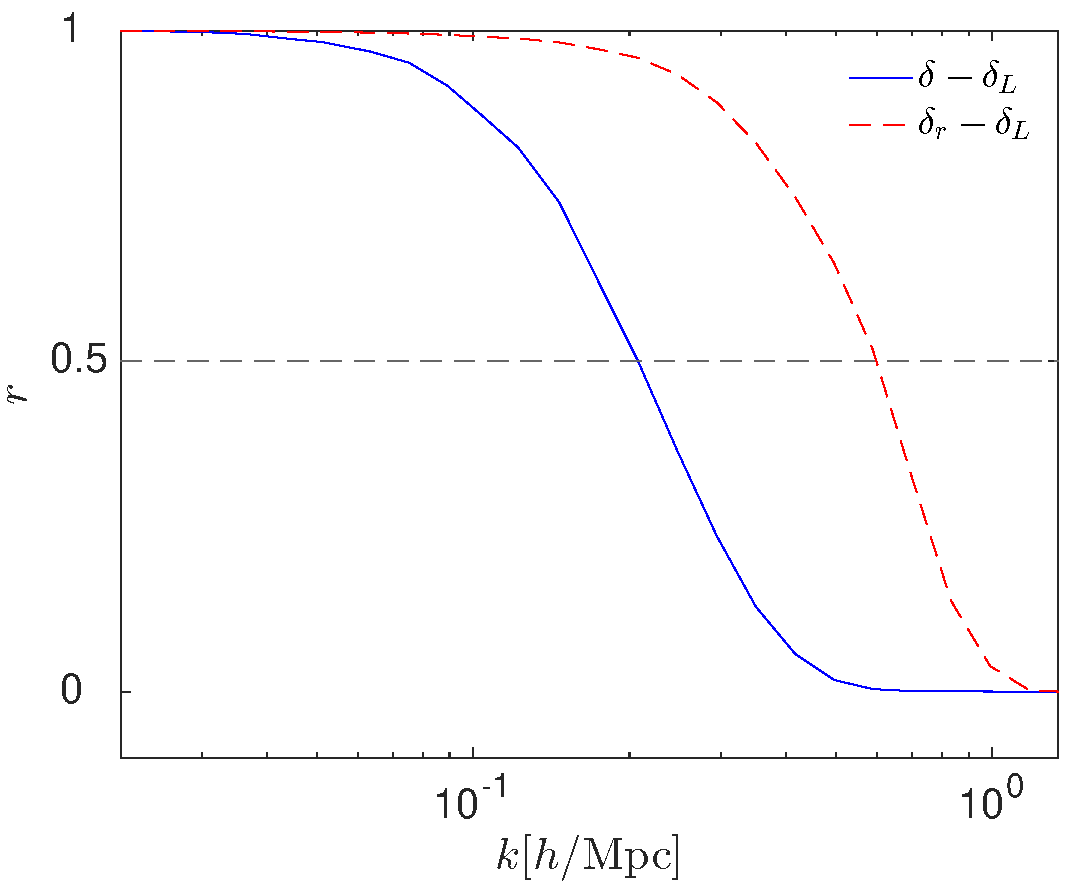
\includegraphics[width=0.48\textwidth]{cross-correlation_analysis-crop.pdf}
%\includegraphics[width=0.5\textwidth]{power_nberror-crop.pdf}
\caption{Cross correlation function $r(\delta,\delta_L)$ (blue line) and $r(\delta_r,\delta_L)$ (red dash line).}
\label{fig:cross-correlation}
\end{figure}
%\begin{subfigure}[b]{0.48\textwidth}
\\begin{figure}[t!]
\centering
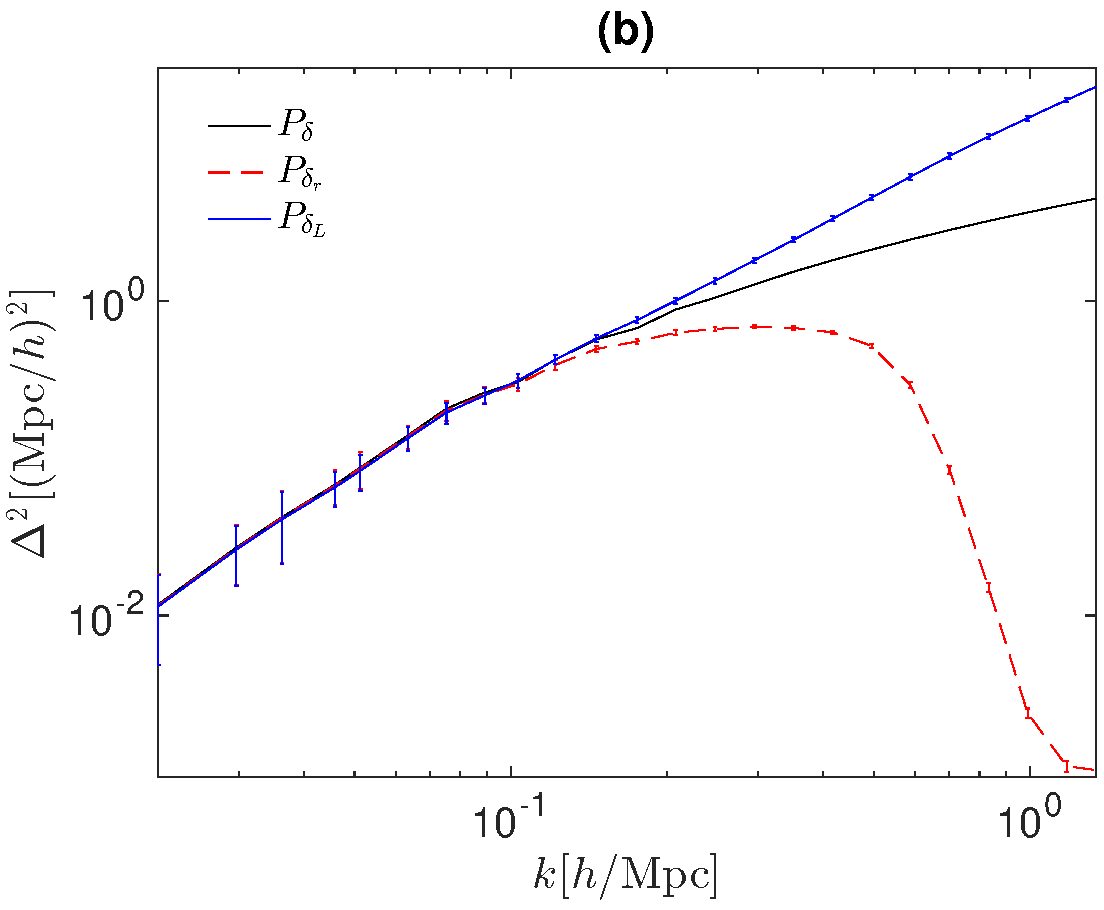
\includegraphics[width=0.48\textwidth]{power_analysis-crop.pdf}
%\end{center}
%\begin{flushright}
%\includegraphics[width=0.48\textwidth]{correlation_goodunit-crop.pdf}
%\end{flushright}
\caption{Linear power spectrum given by transfer function (black line), mean power spectrum with error bar of 
136 non-linear density fields (blue line) and reconstruced density fields (red dash line)}
\label{fig:powerspectrum}
%\end{sufigure}
\end{figure}

   Mathamatically, Fisher information \cite{bib:Tegmark1997} $I$ in the log of amplitude $A$ of the initial 
matter power spectrum is difined as 
\begin{align}
   I_A \equiv - \langle \frac{\partial ^2 \mathrm{ln \Largr}}{\partial A ^2} \rangle,
\label{eq:fisherdefine}
\end{align}
   in which $\Largr$ denotes the likelihood. For Gaussian fluctuations, the likelihood depends on
parameters only through the power spectrum $P(k)$, and the information $I$ in A defined by (\ref{eq:fisherdefine})
can be written as \cite{bib:Rimes2006}
\begin{align}
    I_A = - \left\langle \sum_{k,k'} \frac{\partial \mathrm{ln} P(k)}{\partial \mathrm{ln} A} 
\frac{\partial ^2 \mathrm{ln \Largr}}{\partial \mathrm{ln} P(k) \partial \mathrm{ln} P(k')}
\frac{\partial \mathrm{ln} P(k')}{\partial \mathrm{ln} A}\right\rangle
\label{eq:fisherdefineforgaussian}
\end{align}
in which the angle bracket denotes the average of all the power spectra samples.

    For any density field $\delta$, we can conveniently decompose it as
\begin{align}
    \delta (k) = b (k) \delta _L (k) + n (k),
\label{eq:decompose}
\end{align}
in which $\delta_L$ denotes the linear density field. Safely select $b (k)$ and $n (k)$ 
such that the correlation $\langle \delta_l (k) n (k) \rangle$ is zero. Correlating the density field 
$\delta$ and linear density field $\delta_L$,
\begin{align}
   \langle \delta (k) \delta_L (k) \rangle = b (k) \langle \delta_L (k) \delta_L (k) \rangle,
\label{eq:correlating}
\end{align} 
    we obtain
\begin{align}
    b (k) = \frac{P _{\delta \delta_L}(k)}{P_{\delta_L}(k)}.
\label{eq:bofk}
\end{align}
Nonlinear evolution drives $b (k)$ to drop from unity, and generates the noice $n (k)$. 
Correlating the density field $\delta$ and itself, we can write it's power spectrum as
\begin{align}
   P_\delta (k) = \mathcal{D} (k) P_{\delta_L} (k) + P_n (k),
\label{eq:powerdecompose}
\end{align}
where $\mathcal{D}(k) \equiv b^2 (k)$ is the non-liear damping factor, which is $\mathrm{exp}(-k^2 \Sigma^2/2)$ 
in Gaussian BAO damping model. $P_n$ is the mode-coupling term.

   With the help of (\ref{eq:bofk}) and (\ref{eq:powerdecompose}), we can replace the partial derivatives 
$\partial \mathrm{ln} p(k) / \partial \mathrm{ln} A$ in (\ref{eq:fisherdefineforgaussian}) with the square of 
crosscorrelation function $r ^2 (k)$ of $\delta$ and $\delta_L$. the second partial derivative terms in 
\ref{eq:fisherdefineforgaussian}, the Hessian of the vector $\mathrm{ln} P(k)$, has the expectation 
value of the Fisher matrix with respect to the log powers. For linear density fields, the Fisher matrix is 
approximately equal to the inverse of the covariance matrix of power spectrum estimates, which should be diagonal, 
with diagonal elements equal to the number of modes in each wavenumber bin (when considering $\bm{k}$ and $-\bm{k}$ 
as the same mode). Thus we can write down a simpler form of cumulative Fisher information in (\ref{eq:fisherdefineforgaussian}), 
\begin{align}
    I_A \left( < k_n\right) = r^2(k)^{\mathrm{T}} \left[ \mathrm{C^{-1}_{norm}} ( k_i,k_j )\right] r^2(k')( i,j \leq n ) ,
\label{eq:fisherformulaused}
\end{align}
where $\mathrm{C_{norm}}$ is the normalized covariance matrix with size per dimension up to $k_n$, defined as
\begin{align}
    \mathrm{C_{norm}} \left( k,k' \right)=\frac{\mathrm{Cov}(k,k')}{\langle P(k)\rangle\langle P(k)\rangle},
\end{align}
and $r$ is the mean cross correlation of a given density field and linear one as a function of $k$ up to $k_n$. 
It's reliable to define samely as (\ref{eq:fisherformulaused}) for non-linear density fields, 
since the Fisher matrix is approximately the same as that of linear density fields in linear scale. 
The covariance matrix is defined as 
\begin{align}
    \mathrm{Cov}\left(k,k'\right)\equiv \frac{1}{N-1}\sum_{i=1}^{N}\left[ P_i \left( k \right) - 
\langle P \left( k \right) \rangle \right]\left[ P_j \left( k' \right) - \langle P \left( k' \right)\rangle \right],
\end{align}
where angle brackets mean the expected values, and $N$ is the total number of simulations.
    The  correlation matrix, normalized version of the covariance matrix,
\begin{align}
    \mathrm{Corr}\left(k,k'\right)=\frac{\mathrm{Cov}\left(k,k'\right)}{\sqrt{\mathrm{Cov}\left(k,k\right)\mathrm{Cov}\left(k',k'\right)}},
\end{align}
represents the correlation between different $k$ modes. 
The corelation matrices for non-linear and reconstructed power spectra from
reconstructions are shown in Fig. \ref{fig:corrall}. For the non-linear power spectra, the
correlation matrix in linear regime, $k \lesssim 0.2$, is almost diagonal. The off-diagonal elements are produced by 
strong mode coupling in non-linear scale, and super-survey tidal effect which is small in 
linear scale but dominates in the weakly non-linear regime \cite{bib:Kazuyuki2016}.
The correlation matrix for non-linear power spectra has few negetive elements,
 smallest $\mathrm{Corr} \simeq -0.1$, which are produced by the unbiased error and thus 
 will vanish with more simulations \cite{bib:Takahashi2009}.
 For the reconstructed correlation matrix, however, the linear regime expand up to $k \simeq 0.6$, 
but the number and magnitude of negetive off-diagonal elements increase, smallest $\mathrm{Corr} \simeq -0.8$. 

\begin{figure}
 \centering
  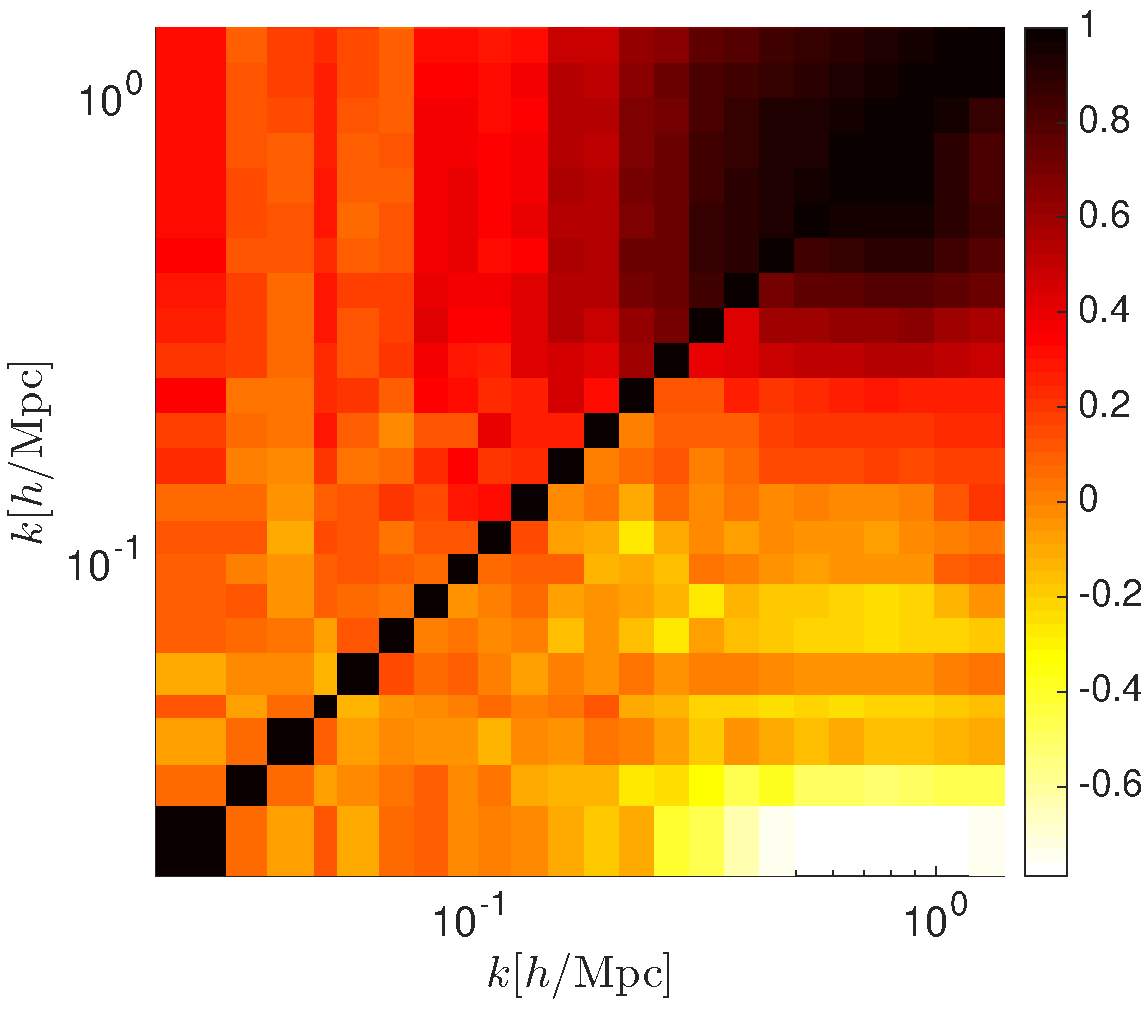
\includegraphics[width=0.48\textwidth]{corrmat_hot-crop.pdf}
%  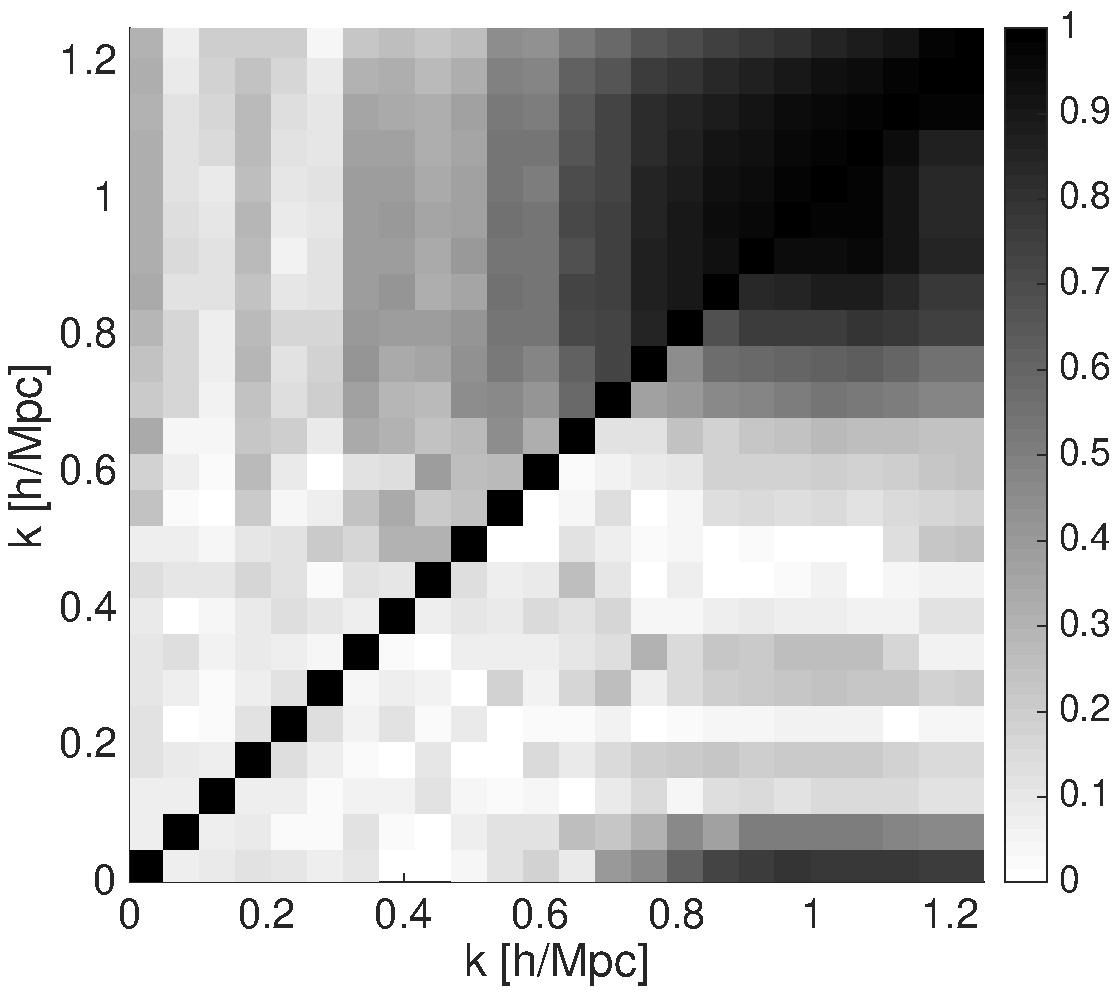
\includegraphics[width=0.48\textwidth]{corr_cut-crop.pdf}
  \caption{Correlation coefficient matrix as found from 136 non-linear power spectra 
(the upper-left elements) and the reconstructed power spectra (the lower-right off-diagonal elements).}
    \label{fig:corrall}
\end{figure}

%  The signal-to-noise ratio, sometimes also called Fisher information, can be given by the inverse matrix of covariance. Since the signal-to-noise ratio was given in some work, we also present it for a better comparison. 
%\begin{align}
%\left( \frac{S}{N}\right)^2 (k_{n}) =\sum_{i,j=1}^n P_i \mathrm{Cov}^{-1}(i,j) P_j
%\end{align}

  We plot the 
cumulative Fisher information of the non-linear, linear and reconstructed power specta in 
Fig.\ref{fig:fisherinfo}(a). The Fisher information of the non-linear power spectra drops 
from the linear one at $k \sim 0.05$, and has a flat plateau in the translinear regime, $k\sim0.3$. It 
indicates that there's nearly no independent information in the translinear regime of the power 
spectrum.
% At $k\sim0.8$, the information increase slightly aggain. 
But the information curve of 
the reconstructed power spectra keeps incresing roughly the same as 
the linear information until $k\sim0.3$, and reaches it's plateau at $k\sim0.8$ 
up to a factor of 40. It indicates that MM reconstructed method can strongly recover the lost information 
within this scale. We compare the Fisher information given by MM reconstruction method with 
logarithmic density mapping method \cite{bib:Mark2009} as an example to illustrate their strength. 
We find that MM reconstruction gives more thatn 10 times more information than logarithmic mapping. 
In some papers, the cross-correlation $r^2$ terms are set to be unity in (\ref{eq:fisherformulaused}), which 
apparantly increases the non-linear information. We also plot those in Fig. \ref{fig:fisherinfo}(b) 
for better comparison. But we find that in this case, the MM reconstructed and logarithmic mapping information in the scale 
$k \sim 0.2 - k \sim 0.5$ is higher than the linear one, which is not expected. 
\begin{figure*}[t!]
%\begin{subfigure}[b]{0.48\textwidth}
%\centering
  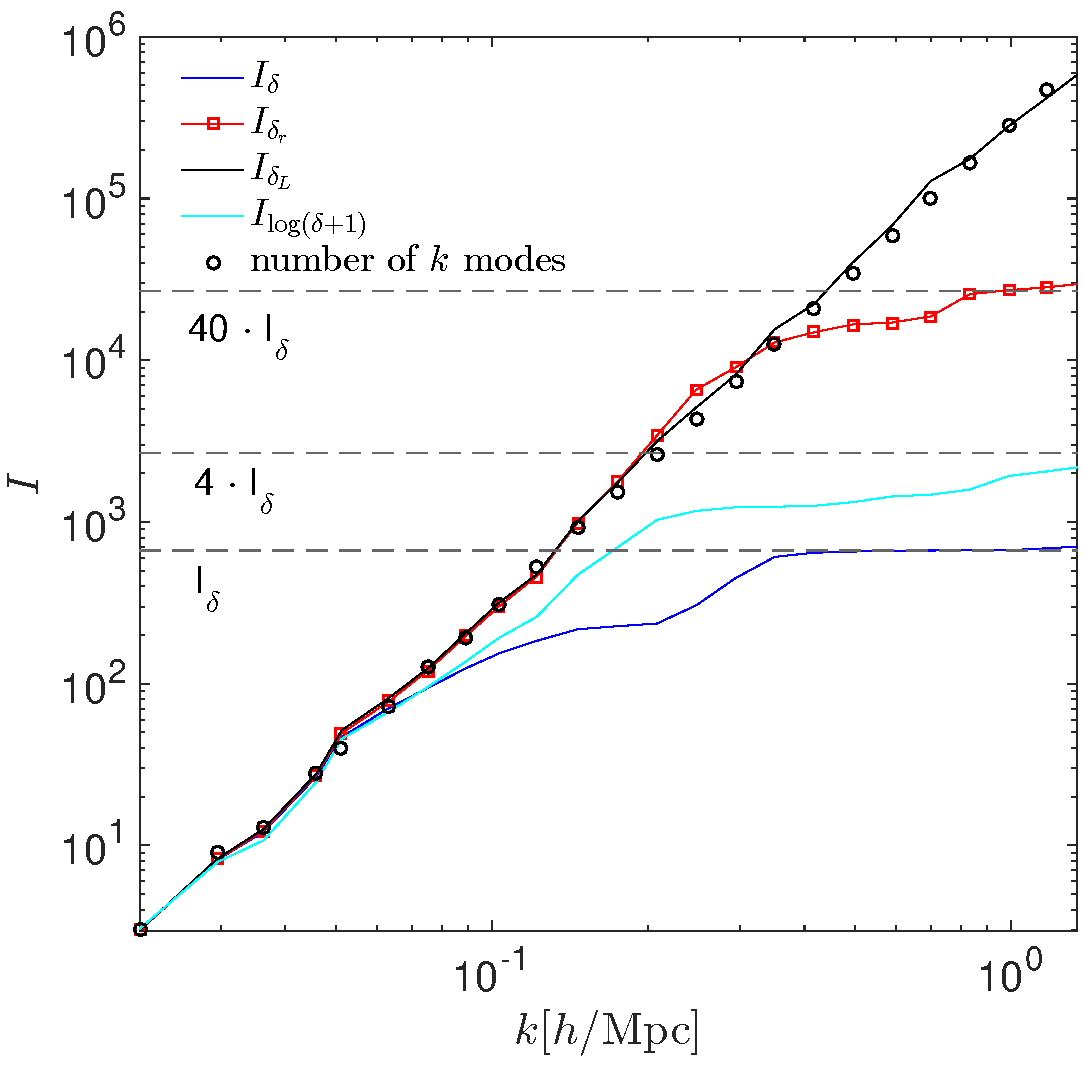
\includegraphics[width=0.48\textwidth]{fisher_addlog_r2_analysis-crop.pdf}
%\end{figure}
%\begin{subfigure}[b]{0.48\textwidth}
%\bebin{subfigure}
%\centering
  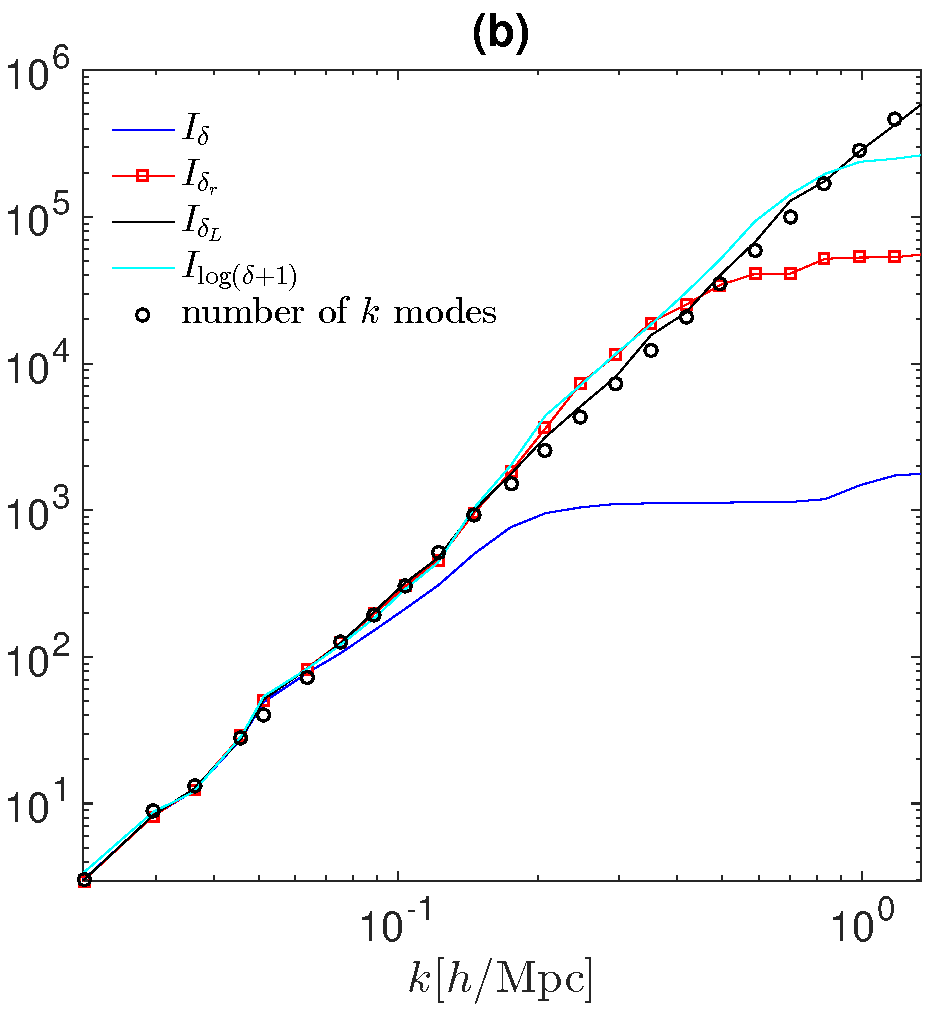
\includegraphics[width=0.48\textwidth]{fisher_addlog-crop.pdf}
%\end{subfigure}
%  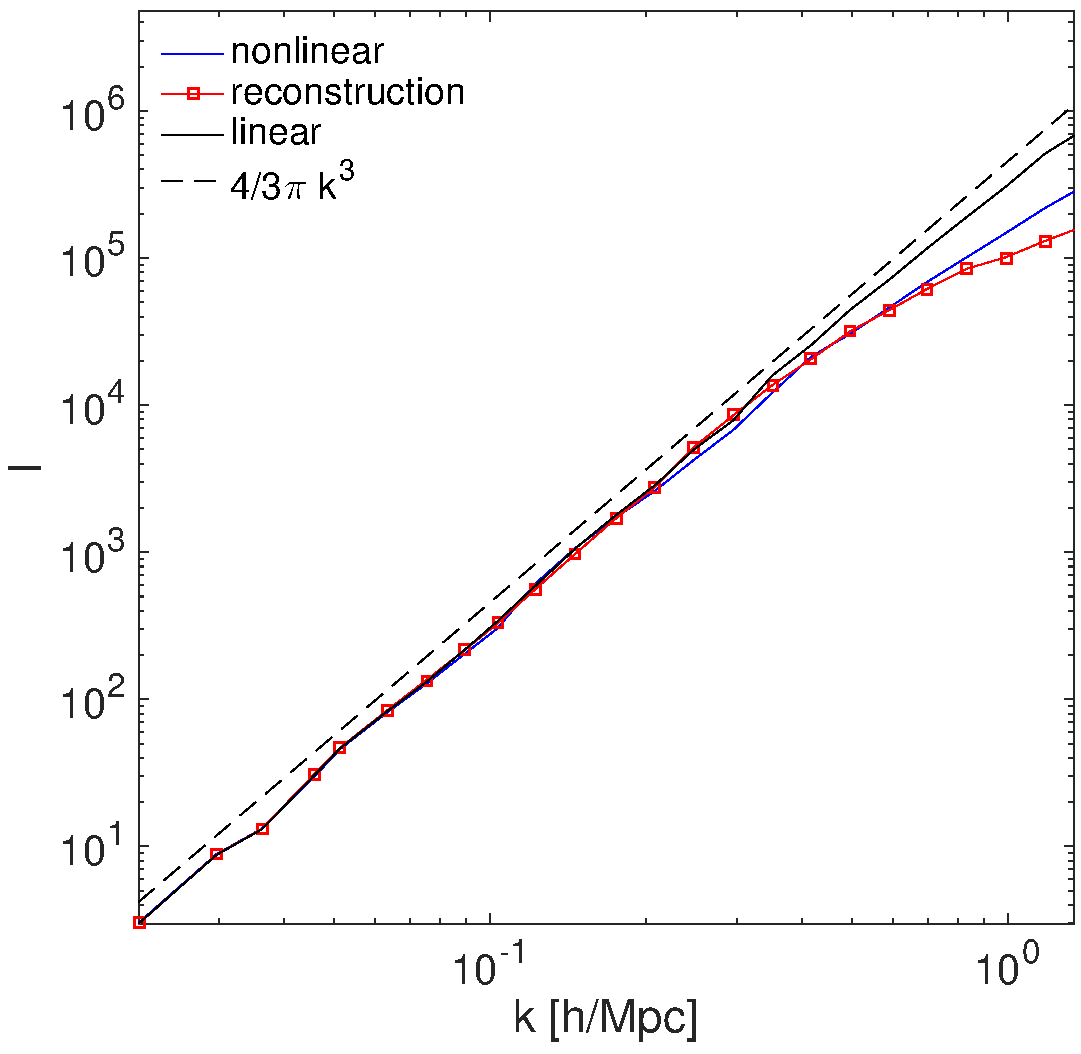
\includegraphics[width=0.48\textwidth]{fisher_tr-crop.pdf}
%  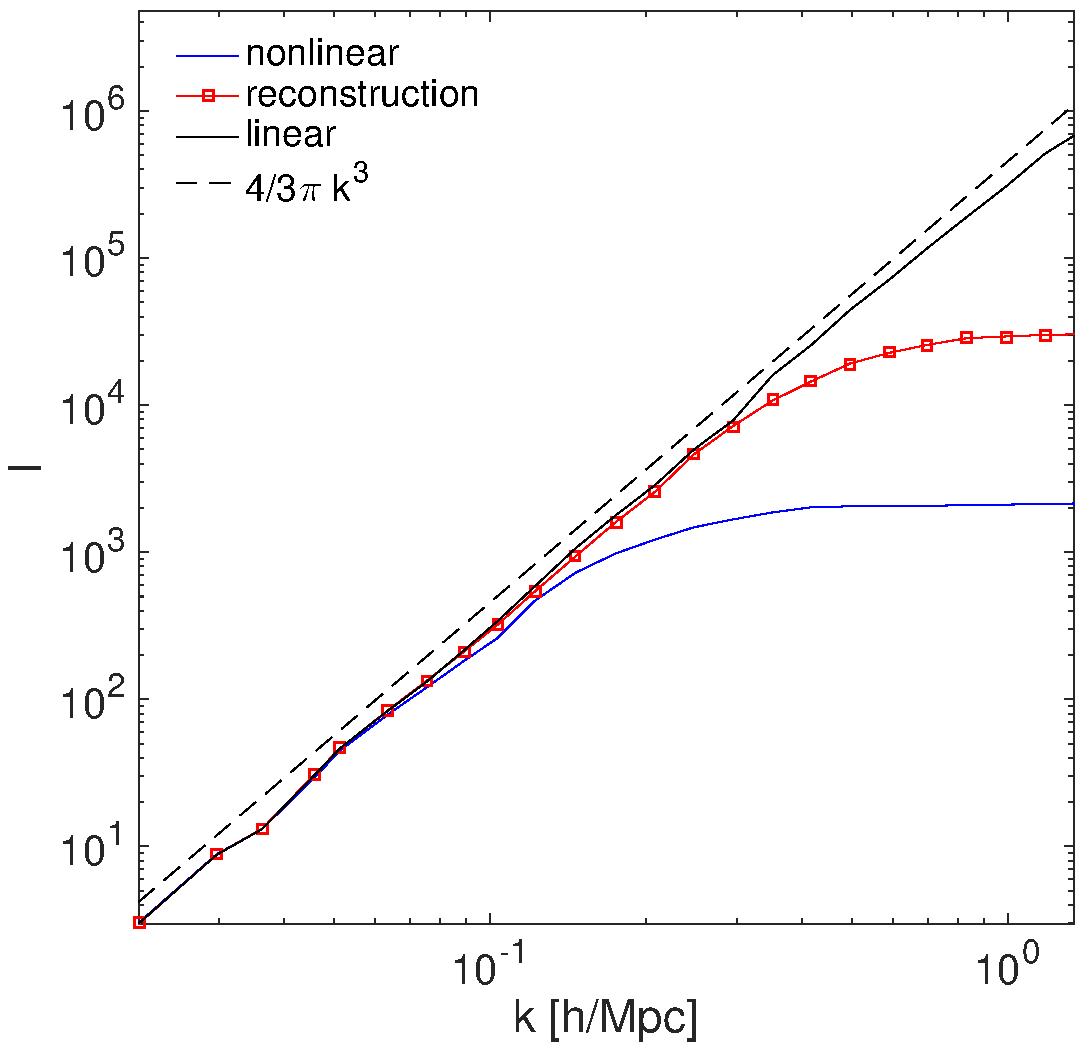
\includegraphics[width=0.48\textwidth]{fisher_trr2-crop.pdf}
\centering
   \caption{(a) Cumulative information in the power spectra as a function of wavenumber. The blue 
line correspond to the non-linear density field by simulation; the red line with squares correspond 
to the the reconstructed deformation potential; the dark line corresponds to linear density 
field; the cycles correspond to number of $k$ modes up to that wave bin. (b) Cumulative information 
given by setting the cross-correlation to be unity.}
  \label{fig:fisherinfo}

\end{figure*}
%\begin{figure*}
%[htbp]
% \centering
%  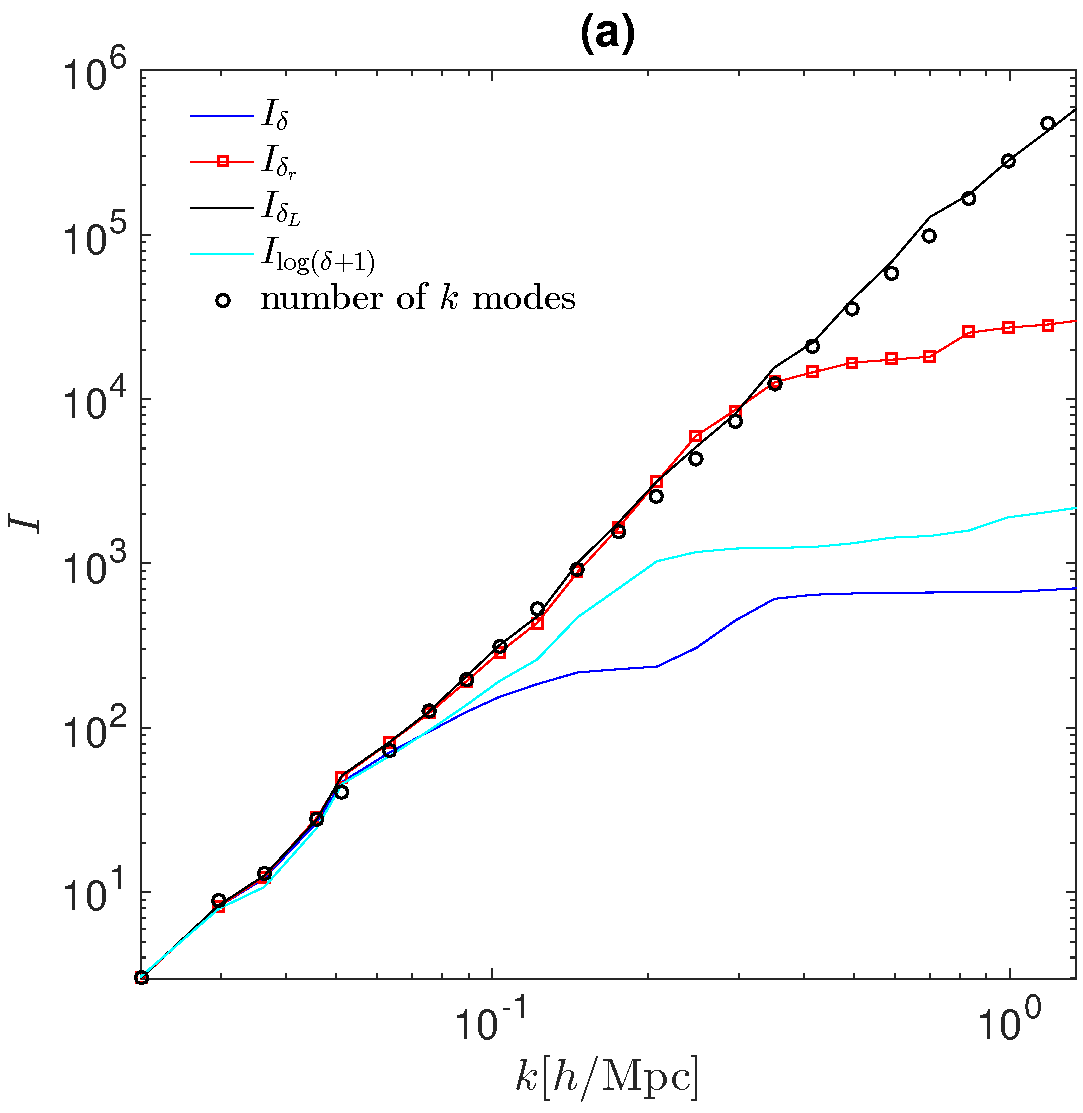
\includegraphics[width=0.48\textwidth]{fisher_addlog_r2-crop.pdf}
%  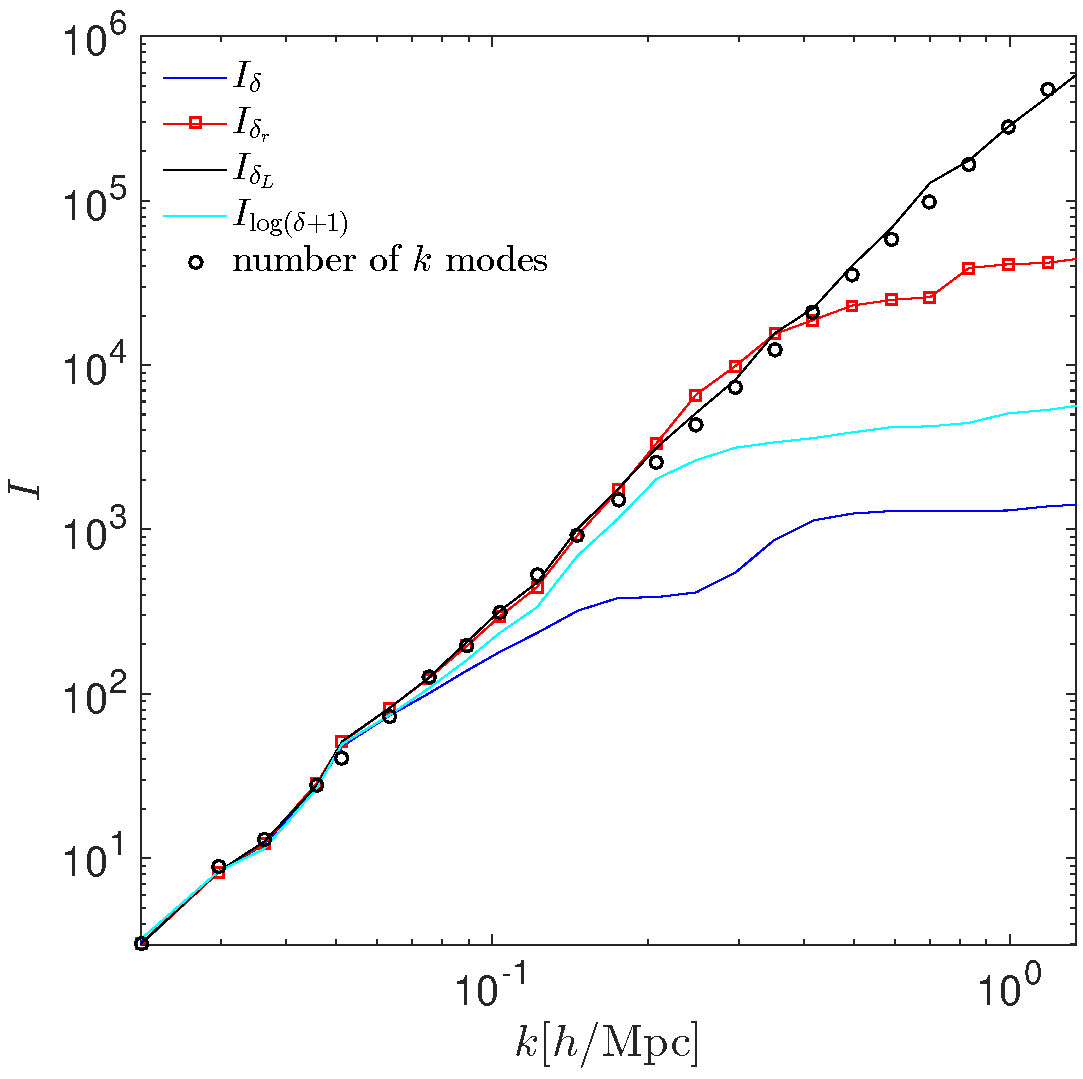
\includegraphics[width=0.48\textwidth]{fisher_addlog_r-crop.pdf}
%  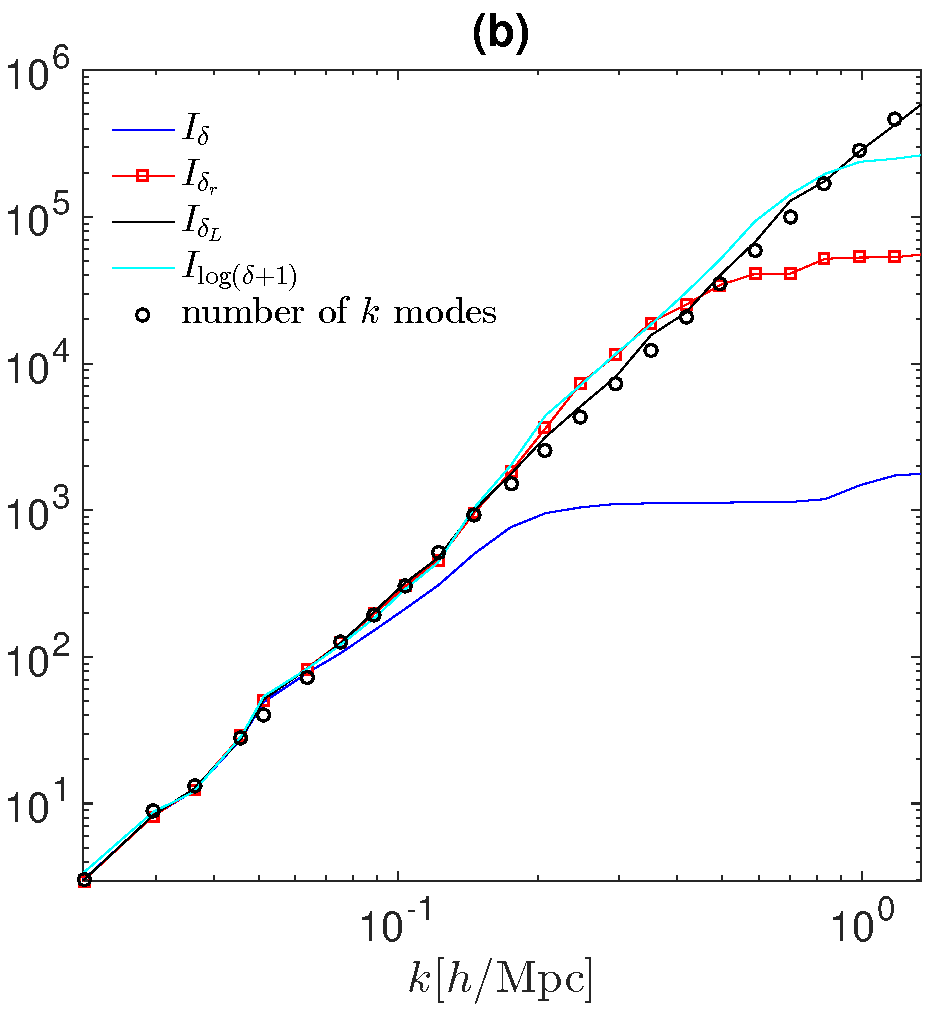
\includegraphics[width=0.48\textwidth]{fisher_addlog-crop.pdf}
%\caption{1:$r^2$; 2:$r$; 3:old version}
%  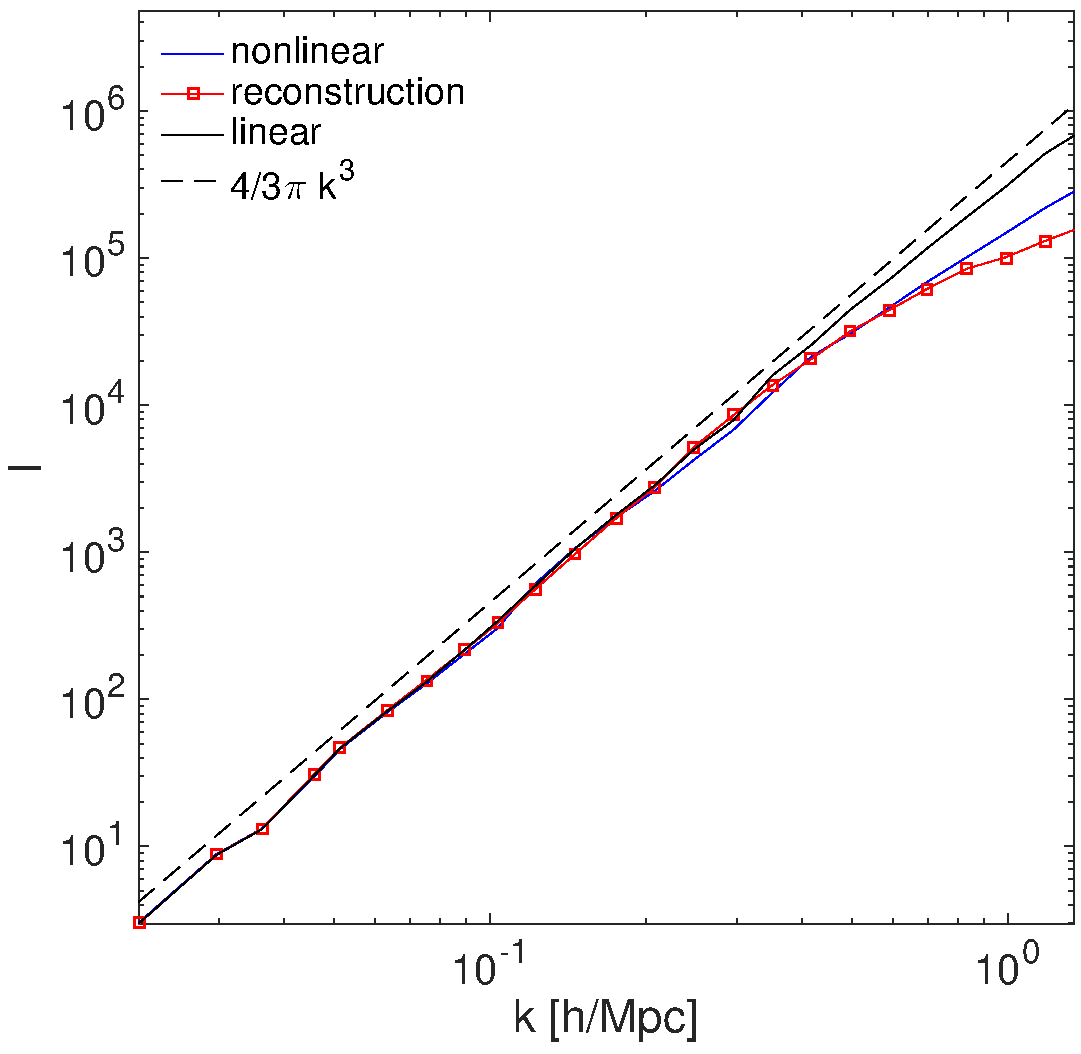
\includegraphics[width=0.48\textwidth]{fisher_tr-crop.pdf}
%  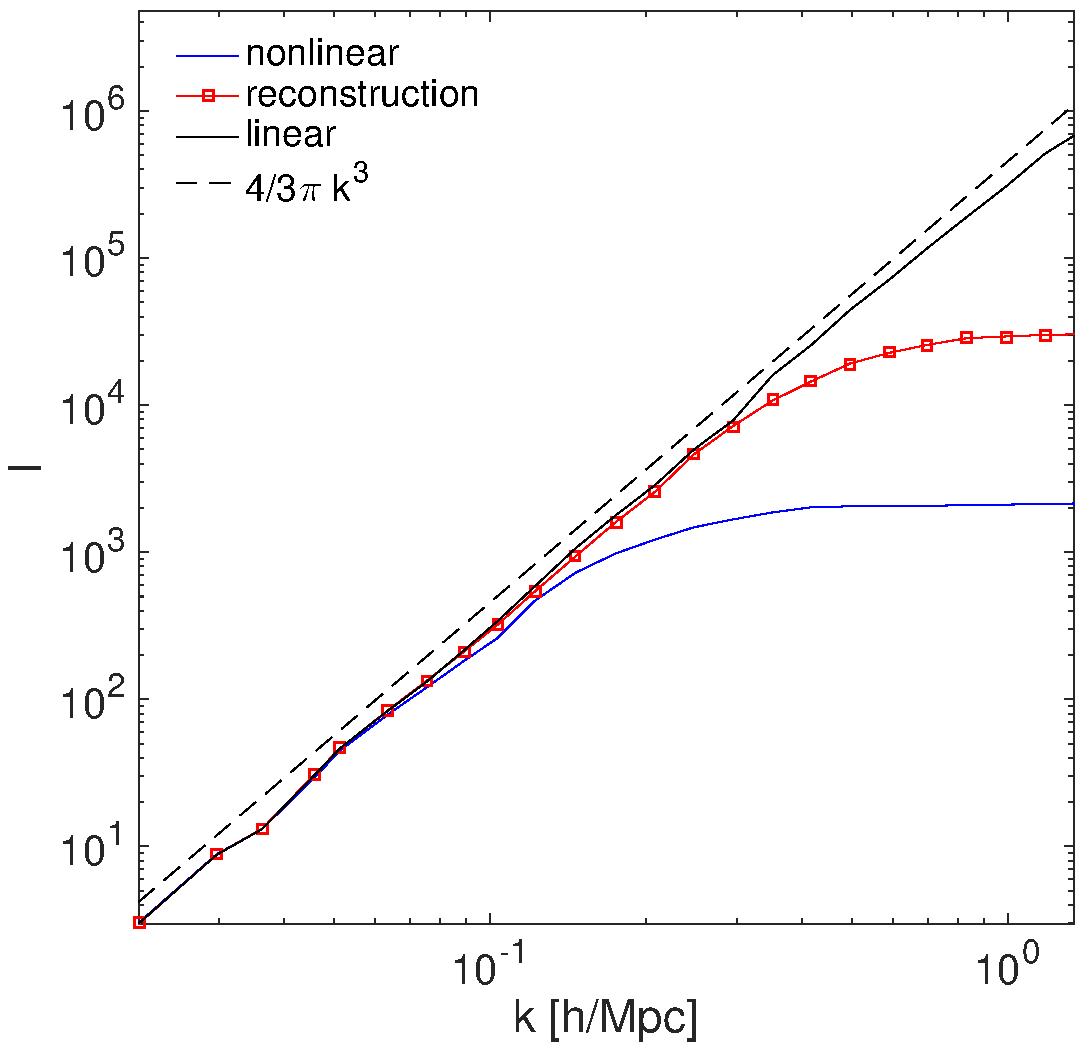
\includegraphics[width=0.48\textwidth]{fisher_trr2-crop.pdf}
%\end{figure*}
%\begin{figure*}
%\centering
%  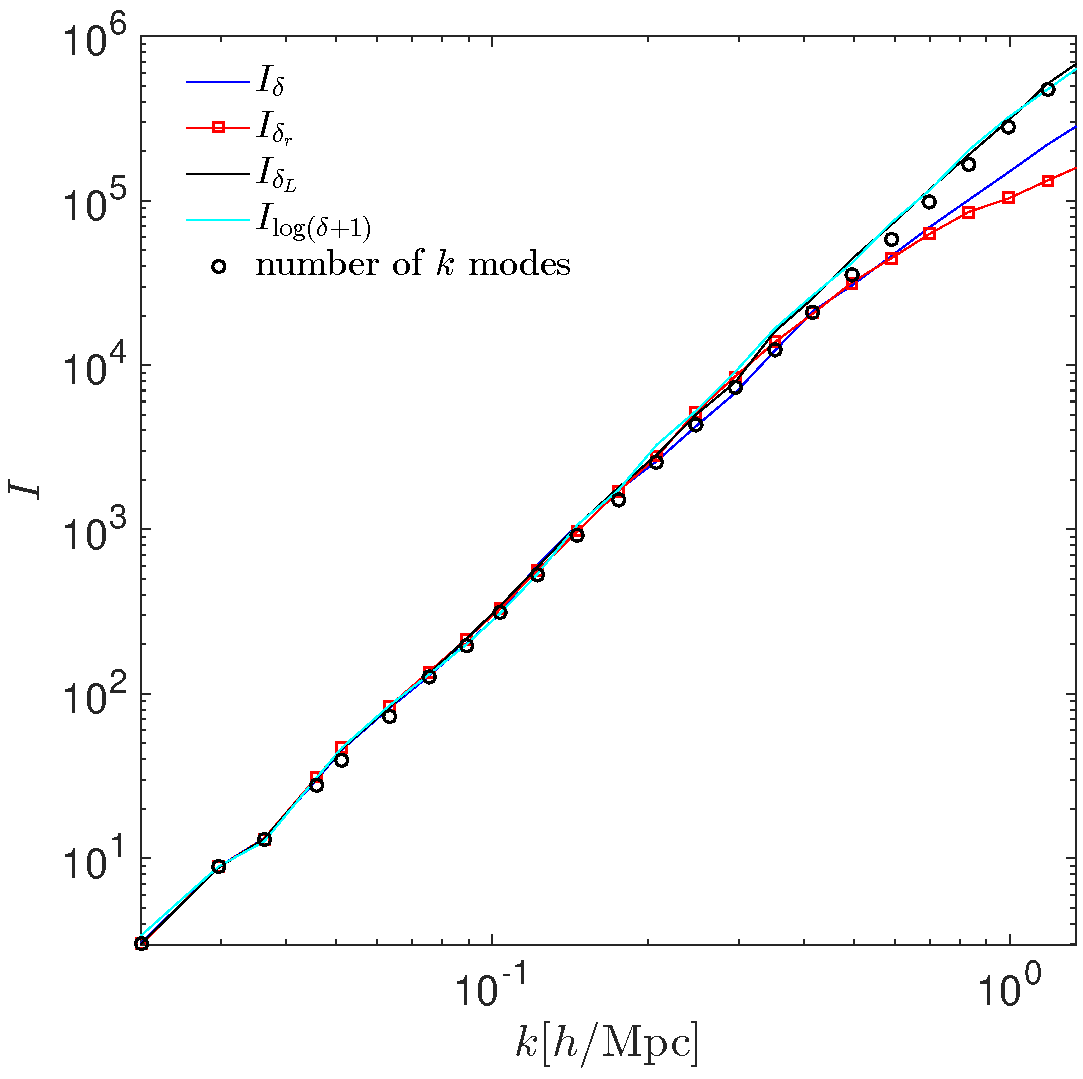
\includegraphics[width=0.48\textwidth]{fisher_addlog_diag-crop.pdf}
%  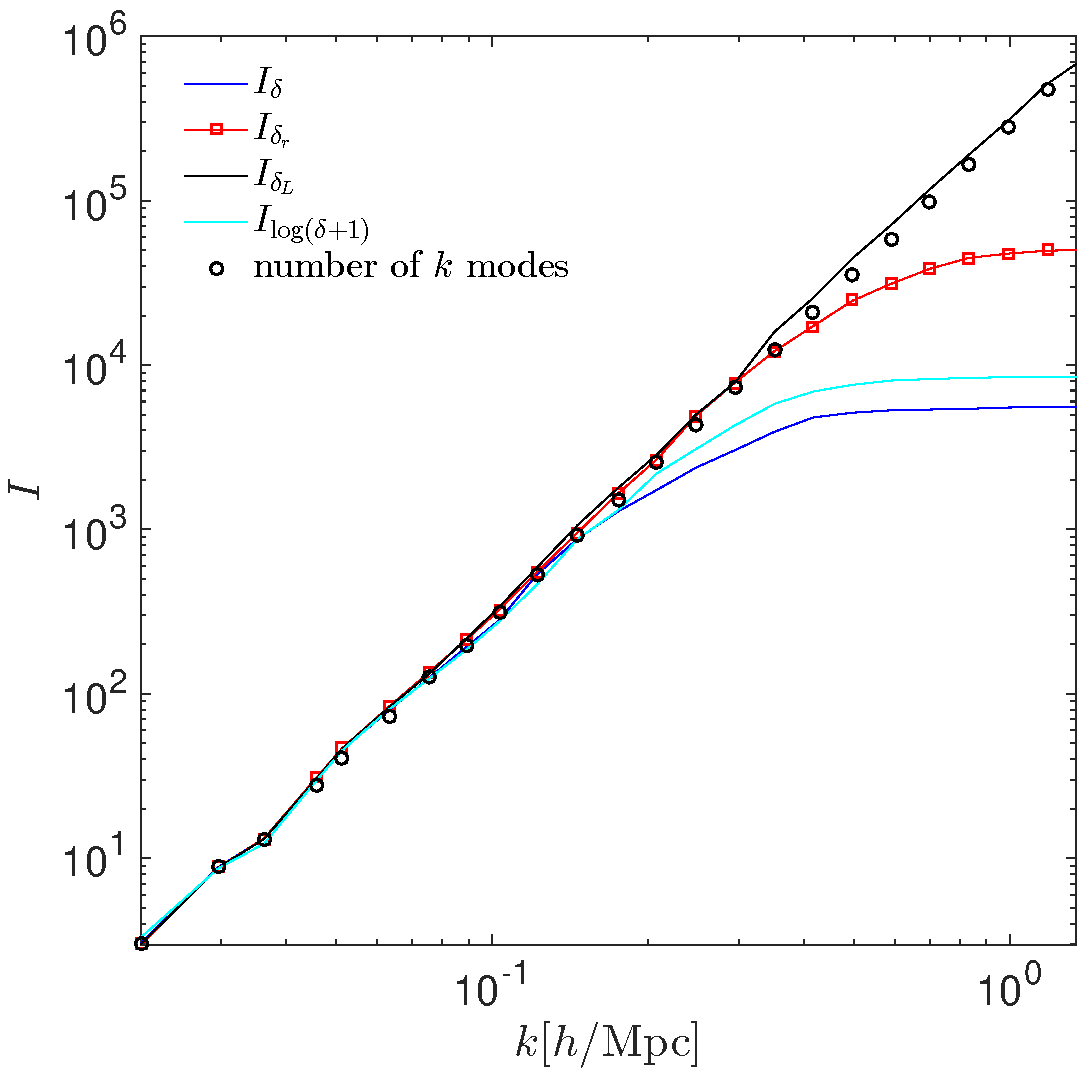
\includegraphics[width=0.48\textwidth]{fisher_addlog_diagr-crop.pdf}
%  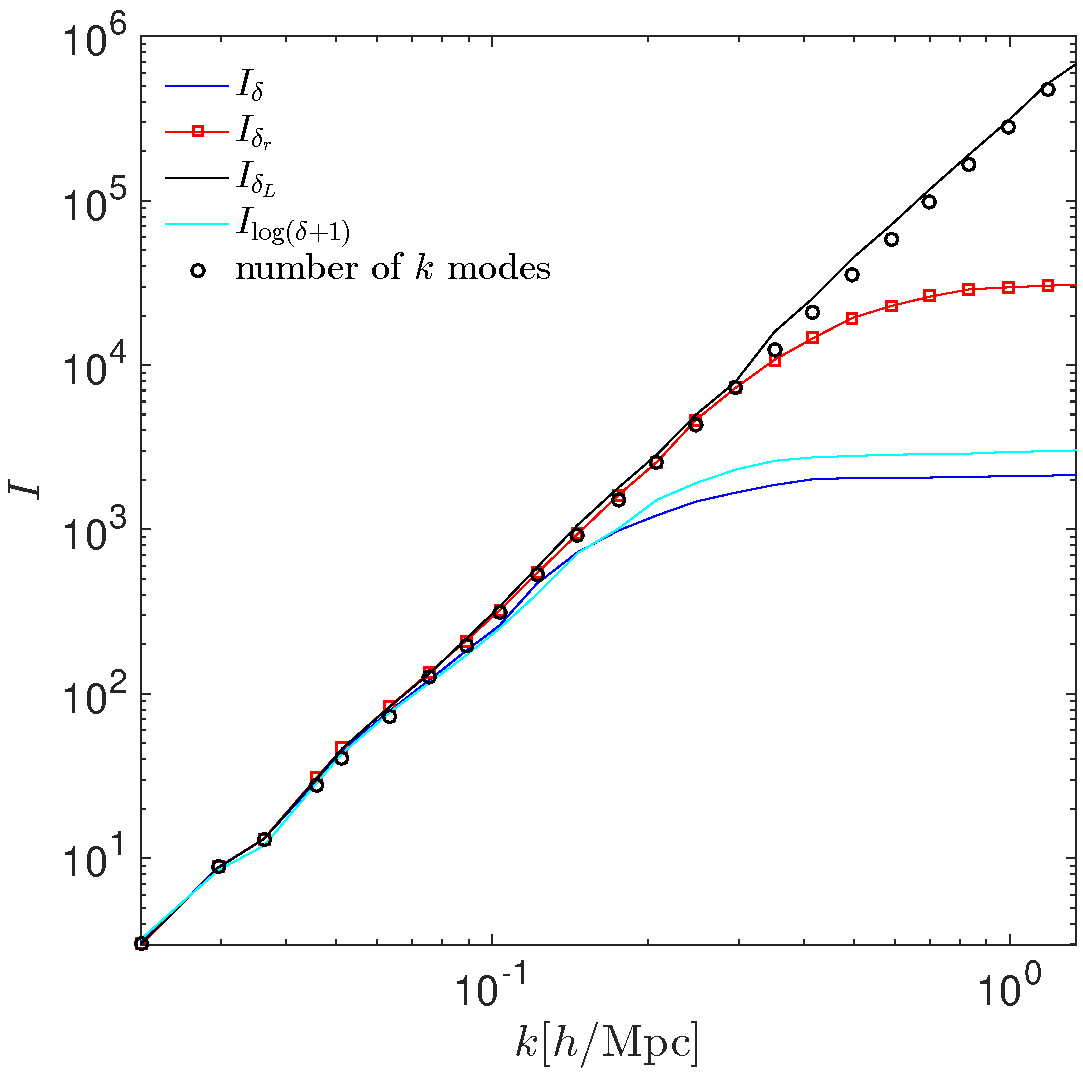
\includegraphics[width=0.48\textwidth]{fisher_addlog_diagr2-crop.pdf}
%\caption{1: diag; 2: diag*$r$, 3: diag*$r^2$}
%\end{figure*}

\end{section}
